\documentclass[11pt, oneside]{report}   	% use "amsart" instead of "article" for AMSLaTeX format
\usepackage[margin = 1in]{geometry}                		% See geometry.pdf to learn the layout options. There are lots.
\geometry{a4paper}                   		% ... or a4paper or a5paper or ... 
%\geometry{landscape}                		% Activate for rotated page geometry
\usepackage[parfill]{parskip}    		% Activate to begin paragraphs with an empty line rather than an indent
\usepackage{graphicx}				% Use pdf, png, jpg, or eps§ with pdflatex; use eps in DVI mode
								% TeX will automatically convert eps --> pdf in pdflatex	
\usepackage{subcaption}									
\usepackage{amsfonts, amsmath,amssymb}
\usepackage{siunitx}
\usepackage[none]{hyphenat}
\usepackage{fancyhdr}
\usepackage{setspace}
\usepackage{hyperref}
%\usepackage[nottoc, notlot, notlof]{tocbibind}		%table of contents
\usepackage{helvet}
\renewcommand{\familydefault}{\sfdefault}

\usepackage{wrapfig}

\usepackage{titlesec}
%\titlespacing\chapter{0pt}{4pt plus 4pt minus 2pt}{4pt plus 2pt minus 2pt}
\titlespacing\section{0pt}{4pt plus 4pt minus 2pt}{0pt plus 2pt minus 2pt}
\titlespacing\subsection{0pt}{4pt plus 4pt minus 2pt}{0pt plus 2pt minus 2pt}
\titlespacing\subsubsection{0pt}{4pt plus 4pt minus 2pt}{0pt plus 2pt minus 2pt}

\titleformat{\chapter}[display]
{\normalfont\huge\bfseries}{\chaptertitlename\ \thechapter}{0pt}{\Huge}
\titlespacing*{\chapter}{0pt}{0pt}{0pt}

\usepackage{sidecap}

\pagestyle{fancy}
\fancyhead{}
\fancyfoot{}
\fancyhead[L]{\slshape \MakeUppercase{4YP Report}}
\fancyhead[R]{\slshape 355136}
\fancyfoot[C]{\thepage}
%\renewcommand{\headrulewidth}{0pt} %remove line in header

\setlength{\parskip}{1em}
\doublespacing

% alternative margin for declaration page
\newenvironment{changemargin}[3]{%
\begin{list}{}{%
\setlength{\topsep}{0pt}%
\setlength{\leftmargin}{#1}%
\setlength{\rightmargin}{#2}%
\setlength{\topmargin}{#3}%
\setlength{\listparindent}{\parindent}%
\setlength{\itemindent}{\parindent}%
\setlength{\parsep}{\parskip}%
}%
\item[]}{\end{list}}


\usepackage{mathtools}
\newcommand\SmallMatrix[1]{{%
  \tiny\arraycolsep=0.3\arraycolsep\ensuremath{\begin{pmatrix}#1\end{pmatrix}}}}
\DeclareMathOperator{\diag}{diag}
%\DeclareMathOperator{\f}{f}




\title{B1 Project Report}
\author{Candidate Number: 355136}
\date{}							% Activate to display a given date or no date

\begin{document}
\pagenumbering{Roman}

\begin{titlepage}
\begin{center}
\vspace*{1cm}
\Large {\textbf{The University of Oxford}}\\
\Large{\textbf{Engineering Science}}\\
\vfill
\noindent\rule{5in}{0.6pt}\\[1mm]
\huge{\textbf{4YP Project Report}}\\[3mm]
\Large{\textbf{- Using Machine Learning to Control Software Synthesisers  -}}\\[1mm]
\noindent\rule{5in}{0.6pt}\\[1mm]
\vfill
Candidate Number: 355136\\
\today\\
\end{center}
\end{titlepage}

%\newgeometry{left=0cm,right=0cm,top=0cm,bottom=0cm}
\begin{changemargin}{-1in}{0in}{-1.5in}
\includegraphics{Declaration_of_Authorship_form_2018.pdf}
\thispagestyle{empty}
\end{changemargin}

\begin{abstract}
\begin{flushleft}
Software Synthesisers (Soft-Synths) are computer applications which create sounds in response to musical input typically in the form of MIDI messages. They are widely used in a variety of musical contexts. Typical soft-synths have hundreds or thousands of parameters which control the sound generation algorithm, allowing the user to create sounds that suit their musical needs. This results in a high dimensional, non-linear search space which the user must navigate in order. Research indicates that humans are bad at navigating such interfaces with serial controls, and that there is a strong link between interface design and the level of creativity that the user with experience when using the interface. \\
This work describes a novel interface designed to help users control synthesisers in a quicker and more intuitive manner. It combines 3 interfaces together: a traditional 'knob and slider' interface, a search space visualisation interface, and an iterative blending interface.

THIS ABSTRACT NEEDS A LOT MORE WORK, WILL WORK ON AFTER WRITING MORE OF THE REPORT
\end{flushleft}
\end{abstract}


%\newgeometry{left=1in,right=1in,top=1in,bottom=1in}
\tableofcontents
%\thispagestyle{empty}
\clearpage
\pagenumbering{arabic}
\setcounter{page}{1}


%%%%%%%%%%%%%%%%%%%%%%%%%%%%%%%%%%%%%%%%%%%%%%%%%%%%%%%%%%%%%%%%%%%%%%%%%%%%%
\chapter{Introduction}
\section{Background Information}
Software Synthesisers (Soft-Synths) are computer applications which create sounds in response to musical input typically in the form of MIDI messages. They are widely used in a variety of musical contexts. Typical soft-synths have hundreds or thousands of parameters which control the sound generation algorithm, allowing the user to create sounds that suit their musical needs. This results in a high dimensional, non-linear search space which the user must navigate in order. Research indicates that humans are bad at navigating such interfaces with serial controls, and that there is a strong link between interface design and the level of creativity that the user with experience when using the interface. \\
This work describes a novel interface designed to help users control synthesisers in a quicker and more intuitive manner. It combines 3 interfaces together: a traditional 'knob and slider' interface, a search space visualisation interface, and an iterative blending interface.
\section{Aims of the project}
Aim to ...


\section{Methodology}
dtsadfdsafdsaf

\chapter{Literature Review}
\section{Previous studies of synthesiser parameter spaces}
Several previous...
\section{Previous attempts of using machine learning to control synthesisers}
There have been several previous attempts...

Talk about the preset blending study, including the parameter freezing.



Talk about the google sample mapping with TSNE (infinite drum machine).

Talk about how taking a sound sample from each preset could be a good way to do the dimensionality reduction interface, but how a parameter based approach is preferable in many ways. Mention which sound metrics would be good to use, and the difficulties involved.
\section{Description of HCI design principles for creative musical interfaces}
A number of guidelines for creative musical interfaces

\section{Principal Component Analysis}
Describe the PCA algorithm, and dicuss the possible extention to using Sparse PCA. 

\section{Principal Component Analysis}
Describe the PCA algorithm, and dicuss the possible extention to using Sparse PCA. 


\chapter{Description of Synthesiser and Image Processing Algorithms}
\section{Synthesiser Algorithm}
\subsection{Description}
In order to develop the synthesiser controller, it was necessary to choose a synthesiser to work with. To remove some of the complexities of interfacing with many commercial synthesisers, a purpose built synth was made to make it as easy as possible to work with the interface, whilst being representative of typical soft-synths available.
The programming language Supercollider was used to create a 6 operator Phase Modulation synthesiser, loosely based on the Yamaha DX7, a very famous synthesiser from the 1980s (CHECK DATE).
 
The synthesis algorithm is based around the FM7 UGen for Supercolldier \cite{UGen}, which implements 6 operators with independent amplitudes and frequencies, whose outputs can be used to modulate the phase of any of the operators. The implementation can be simply described by the following discrete time equation: FIND REFERENCE
\begin{equation}
y_i[t+1] = a_i*sin(2\pi T f_i + \sum_{j = 1}^{6} y_j[t]*m_{ij})
\end{equation}
$T$ is the sampling interval,  $y_i[t]$ is the output of operator $i$ at time $t$, $a_i$ and $f_i$ are the amplitude and frequency of operator$i$ and $m_{ij}$ is a scalar parameter determining the level of phase modulation from operator $j$ to operator $i$. This is a very flexible sound generation algorithm which can create a large number of different sounds. \\
The full synthesiser architecture can be described as follows.\\
 A MIDI Note ON message is received with a musical note number $N$ and a velocity $V$. This triggers the sound generations process for this particular note. the note number $N$ is converted into a base frequency $F$. The frequency of each operator is set using the equation: 
 \begin{equation}
	f_i = F*f_i^{coarse}*(1+f_i^{fine})
 \end{equation}
The coarse frequency parameter $f_i^{coarse}$ for operator $i$ can take discrete values \{0.5, 1, 2, 3, ...\}, allowing the operators to set to different harmonics of the base frequency. The fine frequency parameter $f_i^{coarse}$ for operator $i$ can take any value in the range [0,1], and is used to detune operators away from the perfect harmonic ratios. This is the approach usually taken in typical synthesisers when setting frequencies, as usually the fine frequency values will be very small. REFINE THIS BIT\\
The base frequency F can be continually modulated by the MIDI PitchBend control, and by a vibrato envelope (an exponential ramp from a start frequency and amplitude to an end frequency and amplitude, over a time period in the range [0,20] seconds).\\
The operators' amplitudes $a_i$ are then continuously modulated by two low frequency oscillators (LFOs), and a modulation envelope. LFO A is a zero mean triangle wave oscillator with a frequency in the range [0, 20\si{\hertz}], amplitude in the range [0, 1], and phase spread in the range [0, 1] (a parameter which allows the LFO's initial phase to be randomly varied). LFO B is a zero mean square wave oscillator with a frequency in the range [0, 20\si{\hertz}], amplitude in the range [0, 1], and pulse width in the range [0, 1]. The modulation envelope is an ADSR (Attack-Decay-Sustain-Release) style envelope generator, which is triggered by the MIDI Note ON message.
This can be described by the equation:
 \begin{equation}
 	a_i[t] = (1 + LFO^a[t]*lfo^{a}_i)*(1 + LFO^b[t]*lfo^{b}_i)*(ENV^{mod}[t]*env^{mod}_i + (1-env^{mod}_i))
 \end{equation}
where $LFO^a[t]$ and $LFO^B[t]$ are the LFOs' output values at time $t$, ENV[t] is the modulation envelope's output value at time $t$, and $lfo^{a}_i$, $lfo^{b}_i$, and $env^{mod}_{i}$ are parameters which determine how much operator $i$ is affected by the respective signals.\\
After amplitude modulation with the LFOs and the modulation envelope, the operators are fed into the previously described phase modulation algorithm. The 6 outputs from this algorithm are then mixed together, and multiplied by the Amplitude Envelope to form the output signal: $Y[t] = ENV^{amp}[t]*\sum_{i=1}^{6}y_i[t]*a_i^{output}$, where $a_i^{output}$ is the Output Level parameter for operator $i$, and the Amplitude Envelope is another ADSR Envelope generator, similar to the Modulation Envelope.

All of the synths parameters can be easily adjusted in real time, by sending messages through the Open Sound Control (OSC) protocol, a UDP based protocol for sending messages between applications. CITE UDP

A selection of 35 presets were created for this synth, to give a selection of all the different kinds of 'nice' sounds the synth can make, and to provide data to design the interface with.
\begin{figure}[h] \label{fig:SynthSchematic}
	\centering
	\hspace*{-2cm}
	\includegraphics[width = 7.8in]{SynthSchematic.png}
	\caption{Synthesiser Schematic}
\end{figure}



\subsection{Design choices and justification}
Typical commercial synthesisers have a large number of parameters (Yamaha DX7 - 126 parameters, Omnisphere 2 - several thousand parameters), which can be discrete or continuous, and are usually contrained within a range. Some synthesisers have Modular or Semi-Modular architectures, which allow for a lot of flexibility, but due to the combinational explosion of number of parameter combinations, and difficulty blending between presets, this type of architecture is not addressed in the work.
Some synthesisers use short audio recordings, known as samples, as part of their sound creation algorithm. This creates difficulties blending between presets, so this type of architecture will not be considered in this work. (However both of these type of algorithms would be interesting to try as a follow up work).

The type of synth that this work is aimed at is 'analogue-style' synths, in which there is a medium number of parameters, with a fixed internal routing. 

The synthesiser features a combination of continuous and discrete parameters, all of which are bounded. Common bounds are: $[0, 1]$, $[0, k]$ and $[-k, k]$, where $k \in \mathbb{R}^+ $.

The DX7 was chosen to base the synth off because it is a very famous and powerful synth, but is notoriously difficult to use due to the phase modulation algorithm being very un-intuitive. This means that an improved interface has the ability to open up DX7 programming to a less expert user base. WORK ON THIS

The synthesiser was designed to have access to as wide a range of sounds as possible with as few parameters as possible. For example instead of having a separate envelope generator for each oscillator (as in the Yamaha DX7), only 2 envelopes were included, with a blendable amount per operator. The synth has 96 total parameters, compared to the 126 of the DX7, but it can replicate most of the useful sounds of a DX7. Despite aims to reduce parameter count, there are still many redundant parmaeters in most presets for this synthesiser. For example, if the amplitude of one of the LFOs is set to zero, all of the other parameters to do with the LFO will have no effect on the sound. This is a common feature with synthesisers, and presets a challenge when trying to learn useful information from the parameters.

In Yee King's thesis CITE PROPERLY, a similar FM7 Ugen based Supercollider synthesiser was used, but no envelopes or LFOs were included, so that it was limited to producing sounds with a static timbre. Whilst this had advantages for the timbre mapping approach of the work, it resulted in a synthesiser that was not very representative of ones typically used, as envelopes are such an important part of designing sounds. 





An interesting property of this synthesiser design is that due to the 6 identical operators which can be configured in any combination, there is lots of possible permutation ambiguity, as if two operators have all of their parameters switched, the sound will remain identical. This presents a challenge as two presets can have very different parameters despite having the exact same sound. 
\section{Image Processing Algorithm}
\subsection{Description}
asdasdasda
\subsection{Design choices and justification}
asdasdas

\chapter{Description of Full Interface}
The full interface is a combination of 3 interfaces. Each interface has the ability to vary the entire set of parameters, and produce a wide variety of sounds, but they are designed to complement each other as well as possible. The user can easily move back and forth between the different intefaces, and there are consistent parameter visualtions in all interfaces.
\section{Traditional Interface}
The Traditional Interface is designed to be representative of a typical software and hardware synthesisers. It has a knob or slider for each parameter of the synthesiser, and has interactive visualisations for some parts of the architecture (namely the envelopes and LFOs). The interface is arranged in three seperate pages, two of which are shown in Figure \ref{fig:TraditionalInterface}. 
If the full interface were to be extended to work with any VST, the traditional interface would be replaced by the VST's user interface. 
\begin{figure}[h] 
	\centering
	\hspace*{-0.2cm}
\includegraphics[width = 3in]{TraditionalUI1.png}
\hspace*{0.2cm}
	\includegraphics[width = 3in]{TraditionalUI3.png}
	\caption{Traditional Interface - Screen 1 and 3}
	\label{fig:TraditionalInterface}
\end{figure}

\section{Selection Interface}
Typical Soft-Synths are supplied with a large number of presets, which are usually named and arranged into categories. They are usually displayed in a list which can be searched by name, or split into category. In many soft-synths, each preset is given a set (usually 8) of Macro Controls, which each vary single parameter or combinations of parameters, and aim to give the user a quick way to tweak each preset.\\
The Selection Interface is a new approach to displaying presets, arranging the presets as cells of a 2D voronoi diagram, such that similar presets are close to each other and coloured similarly. The presets can quickly be compared by moving the mouse around the diagram, and presets are selected by clicking on the cells. Once a preset is selected it can be edited by macro controls. 
The presets have been divided into a number of categories. Clicking the category buttons at the top of the interface highlights the selected category, as shown in Figure \ref{fig:PCAInterface}b.\\
Both the 2D spacing of the presets, and the creating of the macro controls is calculated automatically from the set of presets' parameter values using Principal Component Analysis (PCA).

\begin{figure}[h] 
	\centering
	\hspace*{-0.2cm}
	\includegraphics[width = 3.0in]{PCAInterface1.png}
	\hspace*{0.1cm}
	\includegraphics[width = 3.0in]{PCAInterface2.png}
	\caption{PCA Interface - Normal View, and Category Highlight View}
	\label{fig:PCAInterface}
\end{figure}

\section{Blending Interface}
Preset Blending is a somewhat popular approach in synth interface design, where new presets are created by a linear combination of presets. The Blending Interface is an extension of this approach.\\
Three initial presets (A, B, C) are selected, and are placed on the coreners of the triangle in the centre of the interface. As the cursor moves over the interface, a new preset is created as a weighted sum of the 3 presets, based on promixity to the corners. Once the user finds the optimal preset in the space, the user clicks. The preset clicked on then becomes the preset A (I.e is placed on the bottom corner of the triangle), and a new preset B and C are generated. \\
This process is repeated as many times as desired, allowing the user to keep searching through the parameter space.\\
If the user clicks on the 'Pause on Selected Preset Button', they are shown an interactive display of their past preset choices, which they can use to go back to previously selected settings and resume searching. It is also possible to select 3 if the previous presets, and assign them to preset A, B and C.
The user has the option to freeze sections of the parameter space, which helps the search be more fine tuned to their needs.
The colours of the Blending Interface are calculated to be consistent with the Selection Interface.
\begin{figure}[h] 
	\centering
	\hspace*{-0.2cm}
	\includegraphics[width = 3.0in]{BlendingInterface1.png}
	\hspace*{0.2cm}
	\includegraphics[width = 3.0in]{BlendingInterface2.png}
	\caption{Blending Interface - Normal View, and Selection History View}
	\label{fig:BlendingInterface}
\end{figure}

\section{How the Interfaces are Combined}
When the application is started, the Selection interface is displayed first. Once a preset has been selected and possibly modified with the Macro Controls, the user has the option to click the 'Edit Mode' button, which opens the Traditional Interface, allowing the currently selected preset to be further modified. The user can move back to the Selection Interface by clicking the 'Return to Selection UI' button. The varied preset is displayed on the Selection Interface with a marker, attatched to the original preset, which is positioned and coloured to be consistent with the PCA mapping. If the user wants to undo the edits made to the preset they can click the 'Undo Edit' button. In this way the user can move back and forth between the Blending and PCA interfaces as often as desired.\\
Once three presets have been selected, the user has the option of clicking the 'Blend Mode' button which opens the blending interface, and assigns the three seceted presets to A, B and C. The user can then use the blending interface for as long as necessary, and then click the 'Return to Preset Selection' button. This time another marker is created, with dotted lines to the 3 initially selected presets.\\ 
This marker can then be used in the same way as the cells of the voronoi diagram, I.e it can be previewed by clicking, selected by double clicking, can be edited with the Macro Controls or the Traditional Interface. There are a set of parameter visialisations that are diaplayed alongside all of the presets to give the user more feedback into what changes they are making, and to aid in understanding how the synthesis algorithm works.
\begin{figure}[h] 
	\centering
	\hspace*{-1.5cm}
	\includegraphics[width = 7.5in]{CombinedInterface1.png}
	\caption{Combined Interface - PCA view}
	\label{fig:CombinedInterface}
\end{figure}

\chapter{Design and Evaluation of Interfaces}
\section{Traditional Interface}
%\subsection{Detailed Description}
\begin{wrapfigure}{r}{0.5\textwidth}
		\vspace{-30pt}
	\includegraphics[width = 4in]{TraditionalUI2.png}
	\caption{Traditional Interface - Screen 2}
	\label{fig:TraditionalInterface2}
	\vspace{-60pt}
\end{wrapfigure}
This interface was created in the MATLAB App Designer toolbox. As the parameters are varied, they are sent in real time over OSC to the synthesiser.
\subsection{Strengths}
A skilled user can use knowledge of synthesis to construct any preset they can conceive of. The entire parameter space can be searched. For sectional of the synthesiser archececture that are more intuitive, such as the LFOs and envelopes, this works very well.
\subsection{Weaknesses}
Slow serial control of all of the parameters. Even if the user knows exactly what each parameter should be set to, it will still take several minutes to go through all of the 96 knobs and set them to the correct value. Parts of the synthesis architecture are non-intuitive and fiddly to use, In particular the 36 phase modulation routing parameters shown in Figure \ref{fig:TraditionalInterface2}. If the user doesn't know exactly what they want, or how to acheive a particular sound, this interface can be extremely inefficient and frustrating.

\section{Selection Interface}
%\subsection{Detailed Description}
This interface was created as a Matlab 'figure based application'.
\subsection{Global PCA vs Time/Timbre PCA}
The PCA is calculated in two different ways for different sections of the interface. In 'Global PCA', each of the $36$ presets' $96$ parameters arranged in a $36 * 96$ array. PCA is carried out on this array to produce the Global PCA Weights and Scores. 

In Time/Timbre PCA, the $96$ parameters are partitioned into two sets: $72$ which affect timbre, and $24$ which affect variation of the sound over time (I.e all of the envelope and LFO parameters). PCA is then carried out seperately on the resulting  $36 * 72$, and $36 * 24$ arrays to produce the Time PCA Weights, and the Timbre PCA Weights. 

The Global PCA Weights are used for the XY-RGB mapping of the Voronoi diagram, the Global PCA Macros, and for colouring the Blending Interface. The Time/Timbre PCA Weights are just used for the Time/TImbre Macro Controls.

The user is given the option to switch between the Global, and TIme/Timbre Macro Controls, as the global controls allow a greater ammount to the space to be searched, but the Time/Timbre controls can be more understandable. 
The Macro controls are the same for all presets, but centered on the currently selected preset. I.e. they allow a relative change of parameters not an absolute parameter change.

A possible extension to this approach is to allow parameter freezing, as in the blending interface, and have the PCA Macros automatically be recalculated based on the currently unfrozen parameters.
Another possible extension is to create a unique set of macro controls for each preset, which may make macro controls more useful, but at the sacrifice of consistency between presets.

\subsection{PCA + Histogram Equalisation Description}
When using the Global PCA scores to calculate the XY-RGB position of each preset in the Voronoi diagram, there are some undesirable characteristics of the mapping produced. The sizes of the cells varies dramatically, and the majority of the presets usually get compressed into one of the corners, see Figure \ref{fig:histEqBefore} This is because PCA is linear, and so 'outliers' will skew the diagram, so after rescaling to $[0, 1]$ to fit in the diagram, the 'inliers' will be compressed to a smaller range'. A similar effect occurs with the colour mapping, causing many of the colours to be similar to each other minimising the dynamic range of the diagram. (MORE DETAIL HERE WITH REFERENCE). In user interface design, users usually associate larger icons with greater importance, therefore it would be preferable for all the presets to be of a similar size, so as not to give uninteded meaning to particular presets.\\
To fix this issue, a variant of an image processing method known as histogram equalisation (REFERENCE) was used, resulting in the mapping shown in Figure \ref{fig:histEqAfter}.

\begin{figure}
	\centering
	\begin{subfigure}[b]{0.45\textwidth}
		\includegraphics[width=\textwidth]{PCAInterfaceHistEqBefore.png}
		\caption{PCA alone.}
		\label{fig:histEqBefore}
	\end{subfigure}
	~ %add desired spacing between images, e. g. ~, \quad, \qquad, \hfill etc. 
	%(or a blank line to force the subfigure onto a new line)
	\begin{subfigure}[b]{0.45\textwidth}
		\includegraphics[width=\textwidth]{PCAInterfaceHistEqAfter.png}
		\caption{PCA + Histogram equalisation}
		\label{fig:histEqAfter}
	\end{subfigure}
	\caption{Selection Interface before and after Histogram Equalisation}\label{fig:animals}
\end{figure}

The histogram equalisation in one dimension is described in Figure \ref{fig:HistEq}.
\begin{figure}[h] 
	\centering
	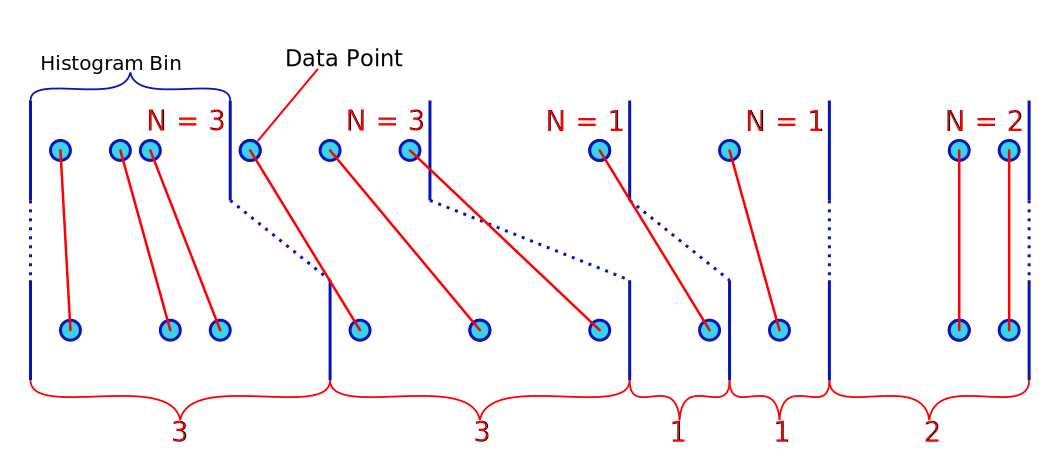
\includegraphics[width = 6in]{HistogramEquilisation.png}
	\caption{Histogram Equalisation}
	\label{fig:HistEq}
\end{figure}
DESCRIBE IN MORE DETAIL


\subsection{Demonstrations of preset group clustering}
asdasdsad
\subsection{Investigate how the PCA mapping scales with number of presets}
asdasdasdsad
\subsection{Quantify the extra variance the macro controls give}
asdasdasdsa
\subsection{Investigate Permutation Ambiguity}
asdasdsa

\section{Blending Interface}
%\subsection{Detailed Description}
This interface was created as a Matlab 'figure based application'.
\subsection{Strengths}
asdsadsa
\subsection{Weaknesses}
asdasdsad
\subsection{Development / Verification using Image Editing Interface}
asdasdsadsa
\subsubsection{Tests of Image Comparison Metric}
asdasdasd
\subsubsection{Convergence Tests for different preset generation algorithms}
asdasdasd
\subsection{Investigate Permutation Ambiguity}
asdasdsad

\section{Comparisons of interfaces}
asdasdsad
\subsection{Perfect /Imperfect User Model}
asdasdsadad
\subsection{Comparison of isolated interfaces}
asdasdsad
\subsection{Comparison of combined interfaces}
asdasdsadsa

\chapter{User tests and Interviews}
asdasdasdsadasd

\chapter{Conclusion}
The interface proposed in this project has many benefits over a traditional synthesiser interface, as has been designed following design heuristics from the fields of Human Computer Interaction and Creative Cognition. Based on simulated user studies, the interface has at least as good performance as a traditional interface when carrying out search based tasks, and based on real user feedback it has many advantages in terms of creativity.
\section{Further Work}
The evaluation of this interface was only carried out on a single synthesiser, due to the projects time constraints. The interface has been designed to be as general purpose as possible, allowing it to control arbitrary synths over the OSC protocol, but due to a lack of standardisation between soft synths, and lack of implementation time, more work needs to be done to create a truly general purpose soft synth controller. As many soft-synths are in the VST format, making a version of the interface with acts as a VST host, and uses the parameter retrieval and preset storage functionality of VSTs is a good next goal if this project is continued in the future.

Talk about how the selections made in the blending interface could be used to create a large dataset of sound preferences, which could be used to train a more sophisticated method of preset generation in the blending interface.

Talk about the hierarchical nature of synthesis parameters could be exploited to improve preset generation and comparison algorithms. 
\begin{thebibliography}{9}
\singlespacing
\bibitem{CleanCode}
Martin, R. (2009). Clean Code. 1st ed. Upper Saddle River, NJ: Prentice Hall, pp.36-52.
\bibitem{WikiLM}
En.wikipedia.org. (2017). Levenberg-Marquardt algorithm. \\
\url{https://en.wikipedia.org/wiki/Levenberg-Marquardt_algorithm}
\bibitem{WikiOp}
En.wikipedia.org. (2017). Optimisation Algorithms \& Methods.
\url{<https://en.wikipedia.org/wiki/Category:Optimization_algorithms_and_methods>}
\bibitem{OOPMatlab}
Introduction to Object Oriented Programming in Matlab\\
\url{https://uk.mathworks.com/company/newsletters/articles/introduction-to-object-oriented-programming-in-matlab.html}
\bibitem{UGen}
Stefan Kersten. skUG SuperCollider UGen library., 2008. \url{http://space.k- hornz.de/software/skug/}.
\end{thebibliography}
\end{document}  